\documentclass[11pt,onecolumn]{article} %twocolumn

\usepackage{tikz}
\def\checkmark{\tikz\fill[scale=0.4](0,.35) -- (.25,0) -- (1,.7) -- (.25,.15) -- cycle;} 

%opening
\title{Twitter Sentiment Analysis with Neural Networks\\or\\ How to Build Neural Networks For Dummies}
\author{Pedro M. Sosa \& Shayan Sadigh}

\begin{document}

\maketitle

\begin{abstract}
\textbf{[TODO]}
\end{abstract}

\section{Introduction: Problem \& Motivation}
Neural Networks are becoming an increasingly common approach to solve Machine Learning problems. \textbf{[TODO: More stuff about NNs]}. This paper aims to give a solid groundwork for researchers wishing to understand and design their own Neural Networks. Furthermore, we seek to frame these explanations using real world scenarios. In this case our Neural Network's goal will be to extract sentiment analysis from Twitter data. This problem is an active problem that many companies and organizations seek to solve, since it could provide valuable marketing information, better feedback analyses, and tracking of overall client sentiment through the Twitter social media platform.


\section{Building A Feed-Forward Neural Network}
\subsection{Basics}
\textbf{[TODO: Neurons, Weight, Sigmoid Function, etc.]}
\subsection{Feed Foward Calculation}
\textbf{[TODO: How we calculate the feed foward]}
\subsection{Backpropagation}
\textbf{[TODO: How we do the backpropagation]}

\section{Pre-processing Datasets}
\subsection{Word Embeddings}
Word embeddings are a recently new method of representing words by plotting them on an n-dimensional vectorspace. There are multiple instances of Neural Networks that use Word Embeddings to solve text related problems \textbf{[TODO: Add these source]}. Following the previous examples, we decided to represent the words in our dataset as 32-dimensional arrays. We employed Keras' Word Embedding methods to build these word vectors.

\subsection{Twitter Specific Features}
Although Word Embeddings are a very popular way to deal with text data, they are very generic and don't assume anything from the given text. However, Twitter has very particular features that distinguish it from other text forms. For example, Twitter data can contain Mentions \textit{(@user)} and Hashtags \textit{(\#topic)} that could provide very meaningful. Furthermore, Tweets are only 140 characters long, which might lead people to shorten words in unexpected ways or make more constant the use of emojis. Knowing this, we decided to also test  tweets as a feature vector.

\par While our original feature vector contained multiple different features, we used WEKA \textbf{[TODO: add specific method]} to narrow the features that proved to be more descriptive. The following table shows all the features tested and which were selected:

\begin{center}
	\begin{tabular}{ | l | l || c |}
		\hline
		Feature Name & Description & Selected \\
		\hline
		
		chwd & \# of Characters/ \# of Words & \checkmark \\
		
		exclamation & \# of exclamation marks (!) & \checkmark \\
		
		smile & \# of positive emoticons & \checkmark \\
		
		sad & \# of negative emoticons & \checkmark \\
		
		url & \# of URLs shared & \checkmark \\
		
		ellipsis & \# of ellipsis (...) & \checkmark \\
		
		mention & \# of mentions (@someone) & \checkmark \\
		
		netprob & $\sum_{W \in Tweet} (P_{pos}(W) - P_{neg}(W))$ & \checkmark\\
		
		question & \# of question marks (?) &  -\\
		
		pronoun & \# of pronouns (I, me, mine...) &  -\\
		
		hashtags & \# of hashtags (\#topic) &  -\\
		
		capitals & \# of uppercase letters &  -\\
		
		length & Length of the Tweet &  - \\
			
		\hline
	\end{tabular}
	\newline
	\newline
	\textbf{Table \#1 } - List of features tested. The selected one refer to the the ones used selected through Weka and used in our experiments.
\end{center}

%\subsection{Meta Features}
%\textbf{[TODO: Will you use meta-features such as replies, date and time, etc.]}


\section{Experiments}
Once we had built our own Neural Network and had parsed our dataset into word embeddings and feature vectors we proceeded to test different scenarios to find the best possible configuration. We used a Neural Network built with the python library Keras (with a Tensorflow backend) as the baseline for the following experiments



\subsection{Selecting Parameters}
Our initial experiments consisted on evaluating the best parameter configuration for a Neural Network. These parameters were: batch size, \# of hidden layers, size of hidden layers, and \# of epochs. 
\begin{figure}[t]
\centering
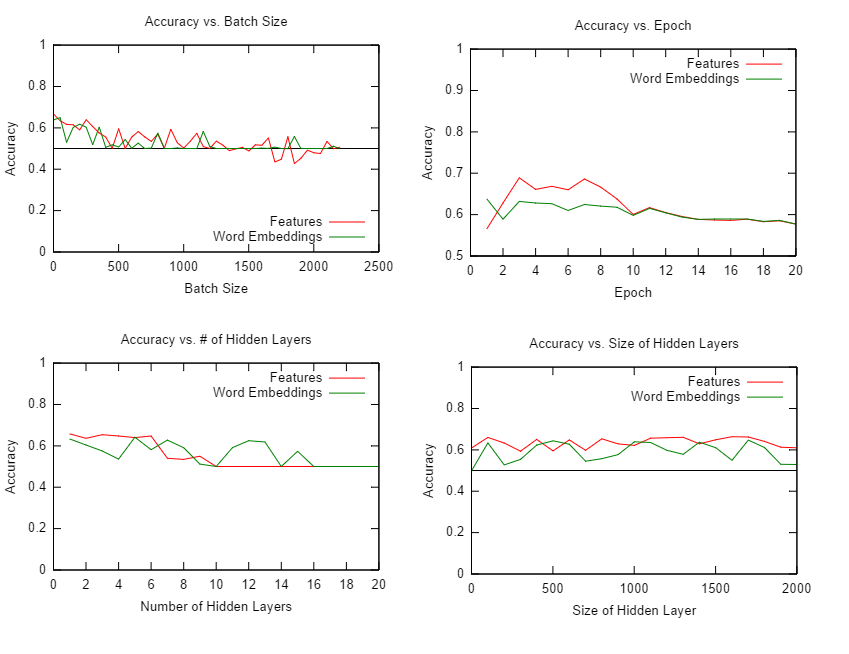
\includegraphics[width=1.1\linewidth]{images/all_in_one}
\caption{}
\label{fig:all_in_one}
\end{figure}

\subsubsection{Batch Sizes}
A Neural Network can be trained with batches of multiple training cases at a time. These batches (also known as minibatches) allow users to cut dataset into smaller segments, feed it through the Neural Network, and update the NN with the mean of the final calculated gradient descent.
\par Having big batches allows the NN to learn from a big dataset faster, as the throughput of each operation is much higher. However, since the update is being done with the mean of the gradient descent of all the batch's training cases, it is possible to loose precision and over-fit to the training data.
\par Our experiments (Figure 1) clearly show that the NN performed better with batches of around 1 - 300 in size. Higher batches tended to converge to a 0.5 or worse accuracy, which could be attributed to over-fitting. 


\subsubsection{\# of Hidden Layers}
It would seem intuitive that the more layers we have the more accuracy we will obtain, since our Neural Network will have an greater ability to recognize different patterns. However, this is not the case, as we increase the number of hidden layers, we find the accuracy of our results drop drastically. This particular behavior commonly refered to as the "vanishing gradient problem" is a typical in Neural Networks that rely on propagation and gradient-based learning.
\par More specifically, this problem happens because during the backpropagation phase, the gradient by which a weight will be updated is calculated using the chain rule. This means that "front" layers will have exponentially smaller update gradients than the "back" layers. In other words, the front-layers train exponentially slower leading to poor results.
\par In our particular experiments, the Neural Network behaved best with 1-2 Layers.

\subsubsection{Size of Hidden Layers}
While increasing the size of a single hidden layer substantially decreased computational performance, it did not seem to affect the accuracy of the NN. However we did see a rise in dead-paths (i.e neural connections with weight = 0). It is important to mention however, that having a hidden layer that was smaller than the size of the input was actually detrimental to the performance while using Features as an input. This might be because the amount of neural paths are so limited that no real features can be distinguished. For the sake of performance, we that an apporpriate size for a layer was around 250-500.

\subsubsection{\# of Epochs}
The number of Epochs refers to the number of times an NN is trained with the same test data. Having multiple repetitions might be useful especially if you have a small training set, however too many repetitions can quickly lead to over-fitting. In our set of experiments we found that the optimum number of epochs was 2-3. Anything past this value, would slowly tend to overfit and thus produce worse results.

\subsection{Word Embeddings vs. Feature Vector}
After selecting the best parameter setup, we tested the Keras NN using both the Feature Vector and the Word Embeddings as inputs. 

\begin{center}
	\begin{tabular}{ | c | c | c | c |}
		\hline
		Batch Size & Epoch & Size of Hidden Layer & \# of Hidden Layers \\
		\hline
		1 & 3 &  250 & 2 \\
		\hline
	\end{tabular}
	\newline
	\newline
	\textbf{Table \#2 } - Selected Parameters for both NN using Word Embeddings or Feature Vectors
\end{center}

\par Table \#3 shows the results of 100 trial runs for each input type (Feature Vector \& Word Embedding) with randomized training and testing data. Our final results show that using a Feature Vector did a slightly better job at describing the tweets than the word embeddings. This might be, as we described before, due to the particular nature of Twitter which motivates users to use emojis, skip whitespace, shorten words in atypical ways, and perhaps include 'typos'. 

\begin{center}
	\begin{tabular}{ | c | c | c | c | c |}
		\hline
		Input Type & Average Acc. & Max Acc. & Min Acc. & Std. Dev. \\
		\hline
		Feature Vectors & 0.6720 & 0.7115 & 0.6330 & 0.0177 \\
		\hline
		Word Embeddings & 0.6140 &	0.6505 & 0.5830 & 0.0150
		\\
		\hline
	\end{tabular}
	\newline
	\newline
	\textbf{Table \#3} - Accuracy results for 100 trial runs of the Keras Neural Network using Word Embeddings or Feature Vector as input.
\end{center}

\subsection{Keras vs. Our Own Neural Network}
\textbf{[TODO]}

\section{Further Work}
While we mostly tested Feed-Foward Neural Networks, there are multiple variations of NNs that could provide a better solution for the Twitter Sentiment Analysis problem. There has been some studies \textbf{[TODO: sources]} that use Convolutional Neural Network to enhance the pattern learning from inputs described with word embeddings. As a final set of experiments we built these NNs with the Keras library and tested them using Word Embeddings as our input.

\subsection{Convolutional Neural Networks}
\textbf{[TODO: Brief explanation of what are Convolutional Networks - Perhaps a pretty picture]}. CNNs have the ability to recognize repeating patterns withing smaller segments of the data. This is specially important with text based problems, as it can pick up phrases or colloquialisms that other simpler NNs would miss. For example, "down to earth" is a phrase that a simple Neural Network might catch as negative, since the word "down" is more commonly used in Tweets to explain negative sentiments. However a CNN could learn that the specific combination "down to earth" is an overall positive phrase. It also has the potential of learning about double negatives and other more complicated linguistic patterns.
\par We found that adding Convolutional layer (with a filter window size of 3 and an overall kernel size of 32) to our original NN would increase the overall accuracy by roughly 2.8\%.


%\subsection{Long Short-Term Memory Recurrent Neural Network}
%\textbf{[TODO: Brief explanation of what are LSTM Networks - perhaps a pretty picture too.]}.


\begin{center}
	\begin{tabular}{ | c | c | c | c | c |}
		\hline
		NN Type & Average Acc. & Max Acc. & Min Acc. & Std. Dev. \\
		\hline
		Original NN & 0.6140 &	0.6505 & 0.5830 & 0.0150 \\
		\hline
		CNN & 0.6421 & 0.6705 & 0.6210 & 0.0134 \\
		\hline
		%LSTM RNN & - & - & - & - \\
		%\hline
	\end{tabular}
	\newline
	\newline
	\textbf{Table \#5} - Accuracy results for 100 trial runs of the different NN programmed with Keras and using Word Embeddings as their input.
\end{center}


\section{Conclusion}
\textbf{[TODO]}
Throughout our different experiments we managed to achieve a \textbf{X}\% accuracy extracting sentiment information from Twitter data. We also elaborated on the pitfalls and problems with solving this particular issue and we explained potential ways of solving them.
Hopefully this work (along with the provided code) could provide a good groundwork for researchers who wish to understand and further engage in the area of Neural Networks and deep learning.

%References
%http://cs.ucsb.edu/~jod//papers/c-12-socialcom2013.pdf

\end{document}